\chapter{\textbf{}} 	%titre entre {} non nécessaire car apparaît deux fois
\begin{center}
\textbf{Titre de l'article} \\
\textit{Journal} (Année), Volume (Issue): pages. \\
Auteurs 
\end{center}

\section{Titre}
\subsection{Titre}
\lipsum[2]

We followed the procedure described by \citet{Siepielski2017} as follow
\begin{align}
  \lambda_{kj} &\sim N(0,\phi^{-1}_{kj}\tau^{-1}_k)\\
  \text{where }  \phi^{-1}_{kj} &\sim \Gamma(2,1)\\
  \text{and }  \tau_k&=\prod^{k}_{l=1} \sim \Gamma(3,1)
\end{align}

In these prior definition, $\lambda$ refers to the parameters of the latent variables, where $\tau^{-1}_k$


%\FloatBarrier
\begin{figure}[htb]
\centering
%\captionsetup{format=hang,justification=raggedright,labelfont=bf, singlelinecheck = false, font=bf, labelsep=quad}
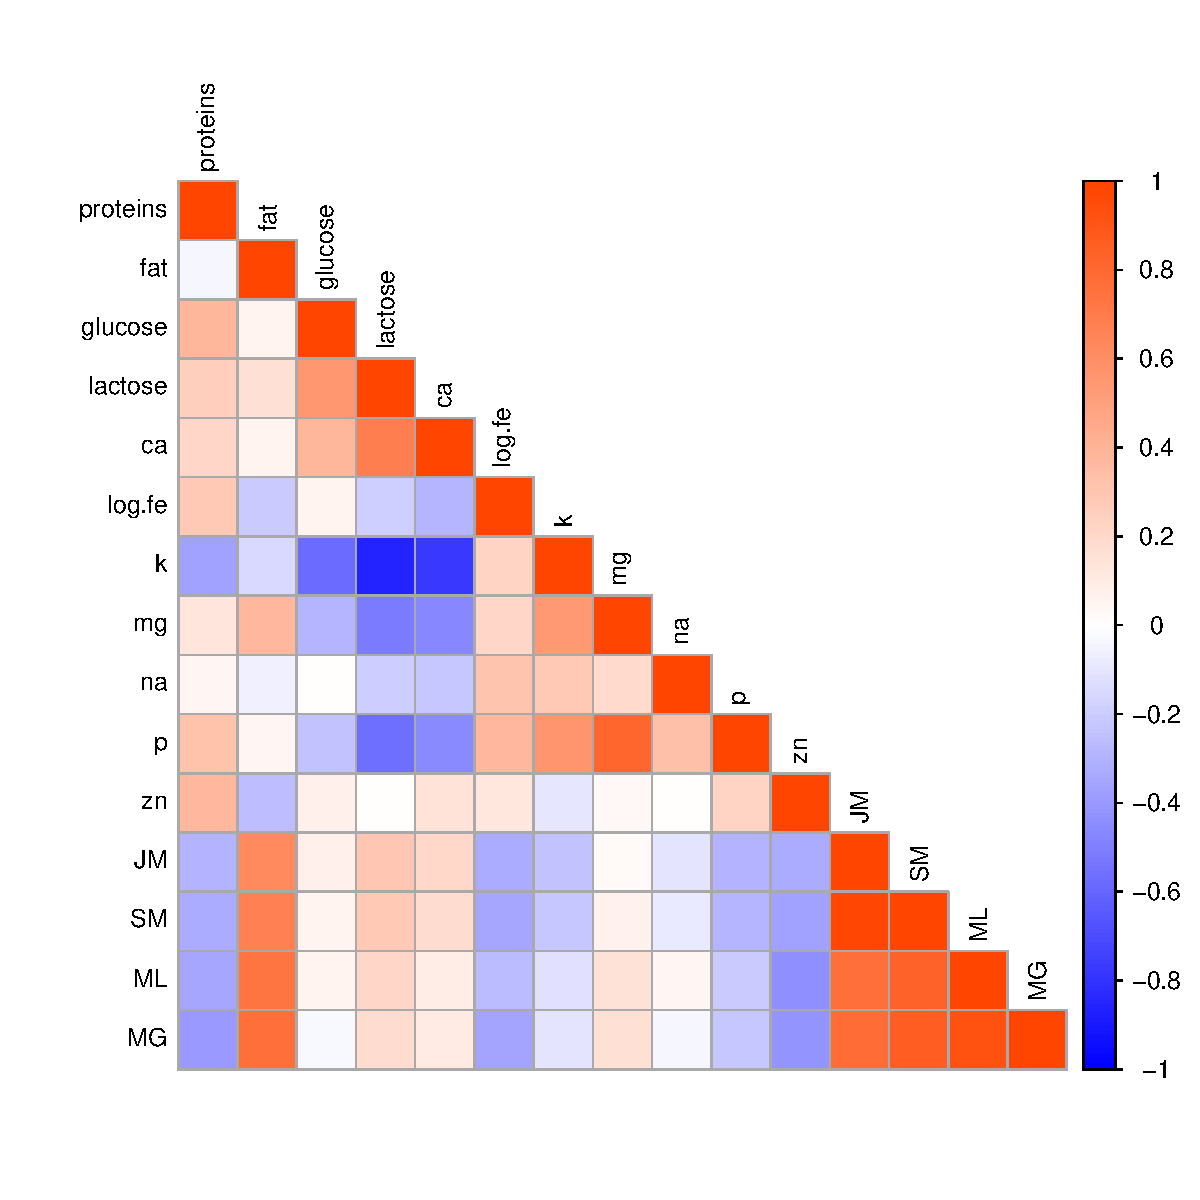
\includegraphics[width=0.85\textwidth]{figs/annexe/ch3/ch3FigS1}
\caption[Titre de figure ]{\label{ch3FigS1}Titre de figure\par{}
\smallskip		% saut de ligne entre titre et légende de figure
\normalfont{
Légende de figure}}
\end{figure}
%\FloatBarrier


% bibliographie pour l'annexe 
\singlespacing
{\renewcommand{\bibname}{References}
\renewcommand{\bibsection}{\section{\bibname}}
\bibliography{bib/chapitre2}
\bibliographystyle{styles/myBEAS} 

